\ifdefined\ishandout
\documentclass[handout]{beamer}
\else
\documentclass{beamer}
\fi

\usepackage[frenchb]{babel}
\usepackage[T1]{fontenc}
\usepackage[latin1]{inputenc}
\usepackage{hyperref}
\usepackage{multirow}
\usepackage{listings}
\usepackage{fancyvrb}
\usepackage{tikz}
\usepackage{framed}
\usepackage{algorithm}
\usepackage{algorithmic}
\usepackage{xcolor}
\usepackage{color, colortbl}
\usepackage{handoutWithNotes}

\usetikzlibrary{shapes.geometric}
\usetikzlibrary{positioning}
\usetikzlibrary{shapes.arrows, chains}
\usetikzlibrary{arrows,calc}
\usepackage{array}
\usetheme{Boadilla}

\ifdefined\ishandout
\pgfpagesuselayout{3 on 1 with notes}[a4paper,border shrink=5mm]
\usecolortheme{dove}
\else
\usecolortheme{dolphin}
\fi


\lstnewenvironment{codeC}
{ \lstset{language=C,
    otherkeywords={printf,scanf}}
}
{}

\ifdefined\ishandout
\definecolor{mygreen}{rgb}{0,0,0}
\definecolor{mymauve}{rgb}{0,0,0}
\definecolor{myblue}{rgb}{0,0,0}
\else
\definecolor{mygreen}{rgb}{0,0.6,0}
\definecolor{mymauve}{rgb}{0.58,0,0.82}
\definecolor{myblue}{rgb}{0,0,1}

\fi

\definecolor{mygray}{rgb}{0.5,0.5,0.5}


\lstset{language=C,
% breakatwhitespace=false,         % sets if automatic breaks should only happen at whitespace
%  breaklines=true,                 % sets automatic line breaking
%  captionpos=b,                
commentstyle=\itshape\color{mymauve},
keywordstyle=\bfseries\color{myblue},
%numbers=left,                    % where to put the line-numbers; possible values are (none, left, right)
%  numbersep=8pt,                   % how far the line-numbers are from the code
%  numberstyle=\tiny\color{mygray}, % the style that is used for the line-numbers
  rulecolor=\color{black},         % if not set, the frame-color may be changed on line-breaks within not-black text (e.g. comments (green here))
%  showspaces=false,                % show spaces everywhere adding particular underscores; it overrides 'showstringspaces'
  showstringspaces=false,          % underline spaces within strings only
%  showtabs=false,                  % show tabs within strings adding particular underscores
%  stepnumber=2,                    % the step between two line-numbers. If it's 1, each line will be numbered
  stringstyle=\color{mygreen},     % string literal style
%  tabsize=2 
}

\newcommand{\red}{\textcolor{red}}
%\newcommand \emph
%Default size : 12.8 cm * 9.6 cm

\newcommand{\tmark}[1]{\tikz[remember picture, baseline=-.5ex]{\coordinate(#1)}}

\ifdefined\ishandout
\newenvironment<>{codeblock}[1]{%begin
  \setbeamercolor{block title}{fg=black,bg=lightgray!80}%
  \begin{block}{#1}}
  % \begin{codeC}}
  %  {\end{codeC}
{  
\end{block}}

\newenvironment<>{termblock}[1]{
    \setbeamercolor{block title}{fg=black,bg=lightgray!90}%
    \begin{block}{#1}
}
%     \begin{Verbatim}}
{%\end{Verbatim}
\end{block}
}

\definecolor{bluegreen}{RGB}{0,0,0}
%\definecolor{bluegreen}{rgb}{0,0.6,0.8}
\else

\newenvironment<>{codeblock}[1]{%begin
  \setbeamercolor{block title}{fg=darkgray,bg=yellow}%
  \begin{block}{#1}}
  % \begin{codeC}}
  %  {\end{codeC}
{  
\end{block}}

\newenvironment<>{termblock}[1]{
    \setbeamercolor{block title}{fg=white,bg=lightgray}%
    \begin{block}{#1}}
%     \begin{Verbatim}}
{%\end{Verbatim}
\end{block}
}

\definecolor{bluegreen}{RGB}{0,149,182}
%\definecolor{bluegreen}{rgb}{0,0.6,0.8}
\fi

%\newcommand{\output}[1]{
\setbeamertemplate{navigation symbols}{}
\newcommand{\bvrb}{\Verb[commandchars=���,formatcom=\color{bluegreen}]}
\newcommand{\footvrb}{\footnotesize\Verb}


%%% Param�tres du cours (� r�gler)
%Num�ro du cours
\newcommand{\nb}{5}

\title[Cours n�\nb]{Cours n�\nb - Les Pointeurs (et les cha�nes de carat�res)}
\author[]{julien.brajard@upmc.fr}
\institute[Polytech' UPMC]{Polytech' UPMC}
\date{17 Octobre 2016}
\begin{document}
%%%%%%%%%%%%%%%%%%%%% SLIDES DE TITRE
\begin{frame}
\titlepage
\centering{
\url{http://australe.upmc.fr} (onglet EPU-C5-IGE Info Gen)}
\end{frame}
%%%%%%%%%%%%%%%%%%%%%
\begin{frame}
\frametitle{Plan du cours n�\nb}
\tableofcontents[hideallsubsections]
\end{frame}

%%%%



%%%%%% SECTION 12
% !TEX encoding = IsoLatin9

%%%%%%%%%%%%%%%%%%%%% SECTION 1
\section{Les cha�nes de caract�res}
\begin{frame}
  \begin{columns}
    \column{4.8cm}
    \tableofcontents[currentsection,hideothersubsections]
    \column{7cm}
    
  \end{columns}
  
\end{frame}

\begin{frame}[fragile]
\frametitle{Les cha�nes de caract�res}
\begin{itemize}
\setlength\itemsep{1em}
\item Les cha�nes de carat�res sont des tableaux
de caract�res ;
\item Chaque case du tableau contient un caract�re ;
\item Le dernier �l�ment est \red{toujours} \Verb|'\0'| ;
\item Pour socker une cha�ne de \Verb|n| �l�ments, il
faut \Verb|n+1| emplacements (� cause du \Verb|'\0'|).
\end{itemize}

\end{frame}

\begin{frame}[fragile]
\frametitle{Initialisation des cha�nes de carat�res}
\begin{block}{}
On peut utiliser les doubles quotes \Verb|"| pour initialiser
une cha�ne de caract�res.
\end{block}

\begin{codeblock}{}
\vspace{-.3cm}
\lstset{escapeinside={��}}
\lstset{basicstyle=\scriptsize}
\begin{codeC}
char tab[] = {'i','n','f','o','r','m','a','t','i','q','u','e','\0'};
\end{codeC}
\vspace{-.3cm}
\end{codeblock}
\vspace{1em}
\centering {ou}
\vspace{1em}
\begin{codeblock}{}
\vspace{-.3cm}
\lstset{escapeinside={��}}
\lstset{basicstyle=\scriptsize}
\begin{codeC}
char tab[] = "informatique";
\end{codeC}
\vspace{-.3cm}
\end{codeblock}
\end{frame}

\begin{frame}[fragile]
\frametitle{Le \bvrb|printf| et les cha�nes de caract�res}

\begin{block}{}
Le formateur de la cha�ne de caract�res dans le \bvrb|printf|
est \bvrb|%s|.
\end{block}
\vspace{1em}

Exemple :
\begin{codeblock}{}
\vspace{-.3cm}
\lstset{escapeinside={��}}
\lstset{basicstyle=\scriptsize}
\begin{codeC}
char tab[] = "informatique";
printf("Nous sommes en cours d'%s\n",tab);
\end{codeC}
\vspace{-.3cm}
\end{codeblock}
\end{frame}

\begin{frame}[fragile]
\frametitle{Saisie de cha�nes de carat�res au clavier}
Il existe deux fonctions en langage C permettant
de saisir des cha�nes de caract�res :
\begin{itemize}
\setlength\itemsep{1em}
\item \bvrb|scanf| (d�j� vu) ;
\item \bvrb|fgets| (sp�cifique pour les cha�nes de caract�res).
\end{itemize}
\end{frame}

\begin{frame}[fragile]
\frametitle{Les \bvrb|scanf| et les cha�nes de caract�res}
\begin{itemize}
\setlength\itemsep{1em}
\item Le formateur de la cha�ne de caract�re dans le
\bvrb|scanf| est \bvrb|%s|.
\item Pensez � d�clarer un tableau de caract�res d'une
taille suffisante avant de l'affecter dans le \bvrb|scanf|.
\item Il ne faut \red{pas} mettre le \bvrb|&|.
\end{itemize}
\begin{codeblock}{}
\vspace{-.3cm}
\lstset{escapeinside={��}}
%\lstset{basicstyle=\scriptsize}
\begin{codeC}
char nom[20];
printf("\n Entrez votre nom : ");
scanf("%s",nom);
printf("\n Bonjour %s !\n",nom);
\end{codeC}
\vspace{-.3cm}
\end{codeblock}

\end{frame}

\begin{frame}[fragile]
\frametitle{Rappel : le caract�re espace}

\begin{block}{}
Le caract�re espace est consid�r� comme un d�limiteur.
La conversion de la m�moire tampon en cha�ne de caract�res
s'arr�te donc � l'espace et ce dernier n'est pas consomm� :
il reste disponible pour la prochaine lecture.
\end{block}

\begin{columns}

\column{0.49\textwidth}

\begin{codeblock}{exemple.c}
\vspace{-.3cm}
\lstset{escapeinside={��}}
\lstset{basicstyle=\scriptsize}
\begin{codeC}
char nom[20];
printf("\n Entrez votre nom : ");
scanf("%s",nom);
printf("\n Bonjour %s !\n",nom);
\end{codeC}
\vspace{-.3cm}
\end{codeblock}

\column{0.45\textwidth}

\begin{termblock}{test 1}
\vspace{-.3cm}
\lstset{escapeinside={��}}
\lstset{basicstyle=\scriptsize}
\begin{lstlisting}
�\textbf{>>}�./exemple
�\color{darkgray}{\texttt{Entrez votre nom : }}� Dupont
�\color{darkgray}{\texttt{Bonjour Dupont ! }}�
\end{lstlisting}
\vspace{-.3cm}
\end{termblock}

\begin{termblock}{test 2}
\vspace{-.3cm}
\lstset{escapeinside={��}}
\lstset{basicstyle=\scriptsize}
\begin{lstlisting}
�\textbf{>>}�./exemple
�\color{darkgray}{\texttt{Entrez votre nom : }}� Dupont toto
�\color{darkgray}{\texttt{Bonjour Dupont ! }}�
\end{lstlisting}
\vspace{-.3cm}
\end{termblock}

\end{columns}
\begin{alertblock}{Conclusion}
Avec \bvrb|scanf| on ne peut pas saisir de cha�ne
de caract�res avec des espaces.
\end{alertblock}

\end{frame}

\begin{frame}[fragile]
\frametitle{Autre solution : \bvrb|fgets|}
\centering{
  \bvrb|fgets(�textit�string�,�textit�taille�,stdin);|
}
\begin{columns}

\column{0.49\textwidth}

\begin{codeblock}{exemple.c}
\vspace{-.3cm}
\lstset{escapeinside={��}}
\lstset{basicstyle=\scriptsize}
\begin{codeC}
char nom[20];
printf("\n Entrez votre nom : ");
fgets (nom,19,stdin) ;
printf("\n Bonjour %s !\n",nom);
\end{codeC}
\vspace{-.3cm}
\end{codeblock}

\column{0.45\textwidth}

\begin{termblock}{test}
\vspace{-.3cm}
\lstset{escapeinside={��}}
\lstset{basicstyle=\scriptsize}
\begin{lstlisting}
�\textbf{>>}�./exemple
�\color{darkgray}{\texttt{Entrez votre nom : }}� Dupont toto
�\color{darkgray}{\texttt{Bonjour Dupont toto ! }}�
\end{lstlisting}
\vspace{-.3cm}
\end{termblock}
\end{columns}

\begin{itemize}
\item Avec \bvrb|fgets|, seule la fin de ligne sert de d�limiteur.
\item \bvrb|�textit�taille�| est le nombre maximum de caract�res
qui peuvent �tre lus.
\item \bvrb|stdin| indique qu'on doit lire les caract�res
dans "l'entr�e standard", c'est � dire dans ce que vous tapez
au clavier. On peut aussi lire les caract�res dans un fichier
(cf cours n$^o$ 7)
\item \red{ATTENTION} : la cha�ne de caract�re lue contiendra le
retour � la ligne.
Dans l'exemple pr�c�dent 
\Verb|nom='D','u','p','o','n','t',' ','t','o','t','o','\n','\0'|
\end{itemize}

\end{frame}

\begin{frame}
\frametitle{�galit� de cha�nes de caract�res}
\begin{block}{}
Pour v�rifier l'�galit� de deux cha�nes de caract�res,
il faut v�rifier un par un tous les caract�res (comme
pour un autre tableau).
\end{block}

\vspace{1em}
\begin{exampleblock}{Exemple :}

Demander � l'utilisateur d'entrer \Verb|pluie| ou \Verb|soleil|,
et afficher "Prenez un parapluie" si l'utilisateur � mis pluie.
\end{exampleblock}
\end{frame}

\begin{frame}[fragile]
\frametitle{La biblioth�que \bvrb|string.h|}
\begin{codeblock}{exemple.c}
\vspace{-.3cm}
\lstset{escapeinside={��}}
%\lstset{basicstyle=\scriptsize}
\begin{codeC}
#include <string.h>
\end{codeC}
\vspace{-.3cm}
\end{codeblock}

\begin{block}{}
Contient des fonctions standards pour g�rer les 
cha�nes de caract�res
\end{block}
Exemples :
\begin{figure}
\centering
\begin{tabular}{|c|p{3.8cm}|}
\hline
Prototype de la fonction & Utilisation \\
\hline
\bvrb|int strcmp(char �textit�s1�[], char �textit�s2�[]);| &
\red{Renvoie}  si les les cha�nes \bvrb|�textit�s1�| et \bvrb|�textit�s2�|
sont �gales.\\
\hline
\bvrb|int strlen(char �textit�s�[]);| & 
Renvoie la taille de \bvrb|�textit�s�|\\
\hline
\end{tabular}
\end{figure}

Pour le d�tail de toutes les fonctions :
\begin{termblock}{}
\vspace{-.3cm}
\lstset{escapeinside={��}}
%\lstset{basicstyle=\scriptsize}
\begin{lstlisting}
�\textbf{>>}� man string
\end{lstlisting}
\vspace{-.3cm}
\end{termblock}
\end{frame}
% !TEX encoding = IsoLatin9

%%%%%%%%%%%%%%%%%%%%% SECTION 1
\section{Adresse et pointeurs}
\begin{frame}
  \begin{columns}
    \column{4.8cm}
    \tableofcontents[currentsection,hideothersubsections]
    \column{7cm}
      \centering{
      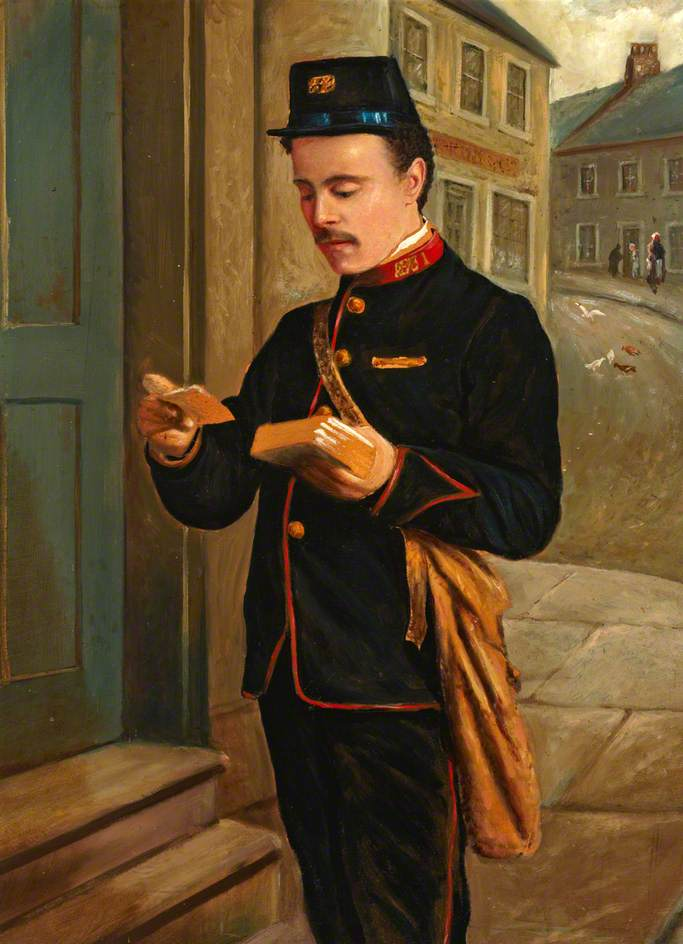
\includegraphics[width=5cm]{fig/postman.jpg}

      \hfill \textit{Portrait of a Postman} (vers 1900-1912 ??)\\
      \hfill Thomas Patterson \\
      \hfill The British Postal Museum \& Archive
    }
  \end{columns}
  
\end{frame}

\begin{frame}[fragile]
\frametitle{Variable et adresse m�moire}
\begin{block}{}
La m�moire d'un ordinateur est organis�e en suite de cases rep�r�es par 
une adresse.
\begin{itemize}
\item Chaque case m�moire a une adresse et un contenu.
\end{itemize}
\end{block}

Les variables d'un programme sont stock�es en m�moire et poss�dent
une valeur.


\begin{columns}
\column{0.2\textwidth}

\begin{codeblock}{}
\vspace{-.3cm}
\lstset{escapeinside={��}}
\lstset{basicstyle=\scriptsize}
\begin{codeC}
int n=3;
\end{codeC}
\vspace{-.3cm}
\end{codeblock}
\end{columns}
\vspace{1em}
\begin{columns}
\column{0.6\textwidth}

\begin{tabular}{|l|c|c|c|c|c|}
\hline
Adresse & ... & 4584 & 4585 & 4586 & ...\\
\hline
Valeur & ... &     & 3 & & \\
\hline
\multicolumn{3}{c}{} & \multicolumn{1}{c}{\Verb|n|}& \multicolumn{2}{c}{}\\
\end{tabular}

\column{0.35\textwidth}
\Verb|n| est � l'adresse 4585

\end{columns}
\end{frame}

\begin{frame}[fragile]
\frametitle{L'op�rateur \textcolor{bluegreen}{\&}}

\begin{block}{}
L'op�rateur \bvrb|&| permet de retrouver l'adresse d'une variable.
\end{block}

\begin{columns}
\column{0.2\textwidth}

\begin{codeblock}{}
\vspace{-.3cm}
\lstset{escapeinside={��}}
\lstset{basicstyle=\scriptsize}
\begin{codeC}
int n=3;
\end{codeC}
\vspace{-.3cm}
\end{codeblock}
\end{columns}

\vspace{1em}
\centering
\begin{tabular}{|l|c|c|c|c|c|}
\hline
Adresse & ... & 4584 & 4585 & 4586 & ...\\
\hline
Valeur & ... &     & 3 & & \\
\hline
\multicolumn{3}{c}{} & \multicolumn{1}{c}{\Verb|n|}& \multicolumn{2}{c}{}\\
\end{tabular}
\vspace{1em}

\begin{tabular}{ll}
\Verb|n| & contient 3 \\
\Verb|&n| & contient 4585 \\
\end{tabular}

\end{frame}

\begin{frame}[fragile]
\frametitle{Les pointeurs}
\begin{block}{}
Un pointeur est une variable contenant l'adresse d'une case m�moire.
\end{block}
\begin{itemize}
\item D�claration :\\
\vspace{0.5em}
\begin{columns}
\column{0.2\textwidth}
\begin{codeblock}{}
\vspace{-.3cm}
\lstset{escapeinside={��}}
\lstset{basicstyle=\scriptsize}
\begin{codeC}
int *pn;
\end{codeC}
\vspace{-.3cm}
\end{codeblock}

\column{0.75\textwidth}
\begin{tabular}{|l|c|c|c|c|c|c|}
\hline
Adresse & ... & 4584 & 4585 & 4586 & ...&6208\\
\hline
Valeur & ... &     & 3 & & &\\
\hline
\multicolumn{3}{c}{} & \multicolumn{1}{c}{\Verb|n|}& \multicolumn{2}{c}{} &\multicolumn{1}{c}{\Verb|pn|}\\
\end{tabular}

\end{columns}

\item Affection :\\
\vspace{0.5em}
\begin{columns}
\column{0.2\textwidth}
\begin{codeblock}{}
\vspace{-.3cm}
\lstset{escapeinside={��}}
\lstset{basicstyle=\scriptsize}
\begin{codeC}
pn = &n ;
\end{codeC}
\vspace{-.3cm}
\end{codeblock}

\column{0.75\textwidth}
\begin{tabular}{|l|c|c|c|c|c|c|}
\hline
Adresse & ... & 4584 & 4585 & 4586 & ...&6208\\
\hline
Valeur & ... &     & 3 & &  & 4585\\
\hline
\multicolumn{3}{c}{} & \multicolumn{1}{c}{\Verb|n|}& \multicolumn{2}{c}{} &\multicolumn{1}{c}{\Verb|pn|}\\
\end{tabular}

\end{columns}

\end{itemize}
\end{frame}

\begin{frame}[fragile]
\frametitle{L'op�rateur \bvrb|*|}
\begin{block}{}
\begin{itemize}
\item L'op�rateur \bvrb|&| permet de retrouver l'adresse d'une variable.\\
\item L'op�rateur \bvrb|*| permet de retrouver le contenu d'une adresse m�moire. (Op�ration de d�r�f�rencement)\\
\end{itemize}
\end{block}
\centering
\begin{tabular}{|l|c|c|c|c|c|c|}
\hline
Adresse & ... & 4584 & 4585 & 4586 & ...&6208\\
\hline
Valeur & ... &     & 3 & &  & 4585\\
\hline
\multicolumn{3}{c}{} & \multicolumn{1}{c}{\Verb|n|}& \multicolumn{2}{c}{} &\multicolumn{1}{c}{\Verb|pn|}\\
\end{tabular}
\vspace{1em}

\begin{columns}
\column{0.27\textwidth}
\begin{tabular}{ll}
\Verb|n| & contient 3 \\
\Verb|pn| & contient 4585
\end{tabular}

\column{0.27\textwidth}
\begin{tabular}{ll}
\Verb|&n| & contient 4585 \\
\Verb|*pn| & contient 3
\end{tabular}

\column{0.35\textwidth}
\begin{exampleblock}{}
Les �galit�s suivantes sont vraies :\\
\Verb|n == *pn|\\
\Verb|pn == &n | 
\end{exampleblock}

\end{columns}

\end{frame}

\begin{frame} [fragile]
 \setbeamercovered{transparent=30}
\frametitle<1>{Manipulation des pointeurs}
\frametitle<2>{Autre Notation}
\begin{columns}
\column{0.3\textwidth}
\begin{codeblock}{}
\vspace{-.3cm}
\lstset{escapeinside={��}}
\lstset{basicstyle=\scriptsize}
\begin{codeC}
int x=1, y=2, z=3 ;
\end{codeC}
\vspace{-.3cm}
\end{codeblock}

\column{0.63\textwidth}
\begin{tabular}{|l|c|c|c|}
\hline
\uncover<1> {Adresse & 2158 & 2159 & 2160} \\
\hline
Valeur &\visible<2>{1}&\visible<2>{2}&\visible<2>{3}\\
\hline
\multicolumn{1}{c}{} & \multicolumn{1}{c}{\Verb|x|}& \multicolumn{1}{c}{y} &\multicolumn{1}{c}{\Verb|z|}\\
\end{tabular}

\end{columns}
\hrulefill


\begin{columns}
\column{0.3\textwidth}
\begin{codeblock}{}
\vspace{-.3cm}
\lstset{escapeinside={��}}
\lstset{basicstyle=\scriptsize}
\begin{codeC}
int *p = &x ;
\end{codeC}
\vspace{-.3cm}
\end{codeblock}

\column{0.63\textwidth}
\begin{tabular}{|l|c|c|c|c|}
\hline
\uncover<1> {Adresse & 2158 & 2159 & 2160 & 2161} \\
\hline
Valeur &\visible<2>{1\tmark{v1}}&\visible<2>{2}&\visible<2>{3} & \visible<2>{\uncover<1>{2158\tmark{p1}}}\\

\hline
\multicolumn{1}{c}{} & \multicolumn{1}{c}{\Verb|x|}& \multicolumn{1}{c}{y} &\multicolumn{1}{c}{\Verb|z|} &\multicolumn{1}{c}{\Verb|p|} \\
\end{tabular}

\end{columns}
\hrulefill

\begin{columns}
\column{0.3\textwidth}
\begin{codeblock}{}
\vspace{-.3cm}
\lstset{escapeinside={��}}
\lstset{basicstyle=\scriptsize}
\begin{codeC}
y = *p ;
\end{codeC}
\vspace{-.3cm}
\end{codeblock}

\column{0.63\textwidth}
\begin{tabular}{|l|c|c|c|c|}
\hline
\uncover<1> {Adresse & 2158 & 2159 & 2160 & 2161} \\
\hline
Valeur &\visible<2>{1\tmark{v2}}&\visible<2>{1}&\visible<2>{3} & \visible<2>{\uncover<1>{2158\tmark{p2}}} \\

\hline
\multicolumn{1}{c}{} & \multicolumn{1}{c}{\Verb|x|}& \multicolumn{1}{c}{y} &\multicolumn{1}{c}{\Verb|z|} &\multicolumn{1}{c}{\Verb|p|} \\
\end{tabular}

\end{columns}
\hrulefill


\begin{columns}
\column{0.3\textwidth}
\begin{codeblock}{}
\vspace{-.3cm}
\lstset{escapeinside={��}}
\lstset{basicstyle=\scriptsize}
\begin{codeC}
*p = 0 ;
\end{codeC}
\vspace{-.3cm}
\end{codeblock}

\column{0.63\textwidth}
\begin{tabular}{|l|c|c|c|c|}
\hline
\uncover<1> {Adresse & 2158 & 2159 & 2160 & 2161} \\
\hline
Valeur &\visible<2>{0\tmark{v3}}&\visible<2>{1}&\visible<2>{3} & \visible<2>{\uncover<1>{2158\tmark{p3}}} \\

\hline
\multicolumn{1}{c}{} & \multicolumn{1}{c}{\Verb|x|}& \multicolumn{1}{c}{y} &\multicolumn{1}{c}{\Verb|z|} &\multicolumn{1}{c}{\Verb|p|} \\
\end{tabular}

\end{columns}
\hrulefill

\begin{columns}
\column{0.3\textwidth}
\begin{codeblock}{}
\vspace{-.3cm}
\lstset{escapeinside={��}}
\lstset{basicstyle=\scriptsize}
\begin{codeC}
p =&z ;
\end{codeC}
\vspace{-.3cm}
\end{codeblock}

\column{0.63\textwidth}
\begin{tabular}{|l|c|c|c|c|}
\hline
\uncover<1> {Adresse & 2158 & 2159 & 2160 & 2161} \\
\hline
Valeur &\visible<2>{0}&\visible<2>{1}&\visible<2>{3\tmark{v4}} &\visible<2>{\uncover<1>{2160\tmark{p4}}} \\

\hline
\multicolumn{1}{c}{} & \multicolumn{1}{c}{\Verb|x|}& \multicolumn{1}{c}{y} &\multicolumn{1}{c}{\Verb|z|} &\multicolumn{1}{c}{\Verb|p|} \\
\end{tabular}

\end{columns}


\begin{tikzpicture}[remember picture,overlay, auto,
 line/.style     = { draw, thick, color=black},
]
\begin{scope} [every path/.style=line]
\path <2-> ($(p1) + (-0.3,0)$) edge[bend right, *->] (v1) ;
\path <2-> ($(p2) + (-0.3,0)$) edge[bend right, *->] (v2) ;
\path <2-> ($(p3) + (-0.3,0)$) edge[bend right, *->] (v3) ;
\path <2-> ($(p4) + (-0.3,0)$) edge[bend right, *->] (v4) ;


\end{scope}
\end{tikzpicture}

\end{frame}

\begin{frame}[fragile]
\frametitle{Autre exemple}

\begin{columns}
\column{0.6\textwidth}
\begin{codeblock}{}
\vspace{-.3cm}
\lstset{escapeinside={��}}
\lstset{basicstyle=\scriptsize}
\begin{codeC}
#include <stdio.h>

int main() 
{
   int u1, u2, v=3;
   int *p1;
   int *p2;
   u1 = 2*(v+5);
   p1 = &v;
   p2 = p1;
   *p2 = 5;
   p2=&u1;
   u2 = 2*(*p1+5);
   *p2=*p2+1:
   printf("\nu1=%d u2=%d v=%d",u1,u2,v);
   return (0);
}
\end{codeC}
\vspace{-.3cm}
\end{codeblock}
\column{0.29\textwidth}
\begin{termblock}{Test d'ex�cution}
%\vspace{-.3cm}
\lstset{escapeinside={��}}
\lstset{basicstyle=\scriptsize}
\begin{lstlisting}
u1=... u2=... v=...
\end{lstlisting}
\vspace{-.3cm}
\end{termblock}


\end{columns}
\end{frame}
% !TEX encoding = IsoLatin9

%%%%%%%%%%%%%%%%%%%%% SECTION 1
\section{Pointeurs et tableaux}
\begin{frame}
  \begin{columns}
    \column{4.8cm}
    \tableofcontents[currentsection,hideothersubsections]
    \column{7cm}
     
  \end{columns}
  
\end{frame}

\begin{frame}[fragile]
\frametitle{Qu'est-ce qu'un tableau}
\onslide<1->{\begin{block}{Point de vue algorithmique}
Un tableau est un ensemble de donn�es de m�me type.
\end{block}}
\onslide<2->{\begin{block}{Point de vue langage C}
Un tableau est un \red{pointeur} sur le premier �l�ment d'un
ensemble de donn�es de m�me type.
\end{block}}

\pause[3]
\begin{columns}
\column{0.64\textwidth}
\centering
\begin{codeblock}{}
\vspace{-.3cm}
\lstset{escapeinside={��}}
\lstset{basicstyle=\scriptsize}
\begin{codeC}
int Tab[4]={5,7,3,2};
\end{codeC}
\vspace{-.3cm}
\end{codeblock}
\begin{tabular}{|l|c|c|c|c|c|c|}
\hline

Adresse & \footnotesize{4583} & \footnotesize{4584} & \footnotesize{4585} & \footnotesize{4586} & ...&\footnotesize{6208}\\
\hline
Valeur & 5\tmark{v} & 7 & 3  & 2 &  & 4583\tmark{p}\\
\hline
\multicolumn{6}{c}{} & \multicolumn{1}{c}{\Verb|Tab|}\\
\end{tabular}

\column{0.3\textwidth}
\begin{exampleblock}{}
Les �galit�s suivantes sont vraies :\\
\Verb|Tab == &Tab[0]|\\
\Verb|*Tab == Tab[0]| 
\end{exampleblock}


\end{columns}



\begin{tikzpicture}[remember picture,overlay, auto,
 line/.style     = { draw, thick, color=black},
]
\begin{scope} [every path/.style=line]
\path ($(p) + (-0.3,0)$) edge[bend left, ->] (v) ;


\end{scope}
\end{tikzpicture}
\end{frame}

\begin{frame}[fragile]
\frametitle{Allocation dynamique de m�moire pour un tableau}
\begin{block}{Allocation}
On peut affecter dynamiquement la m�moire d'un tableau :
\begin{itemize}
\item fonction \bvrb|malloc| de la biblioth�qe \bvrb|stdlib.h| :\\
\bvrb|�textit�nom_pointeur� = (�textit�type�*)malloc(�textit�espace_memoire�);|
\item \bvrb|espace_memoire| = \red{taille du tableau $\times$ taille du type}
\end{itemize}
\end{block}
Exemple pour un tableau de 10 entiers :
%\centering
\begin{codeblock}{}
\vspace{-.3cm}
\lstset{escapeinside={��}}
%\lstset{basicstyle=\scriptsize}
\begin{codeC}
int *Tab ;
Tab = (int *) malloc (10*sizeof(int));
\end{codeC}
\vspace{-.3cm}
\end{codeblock}

\begin{block}{Lib�ration}
Lorsque la m�moire n'est plus utilis�e, il faut penser � la lib�rer :
\bvrb|free(�textit�nom_pointeur�);|

\end{block}



\end{frame}

\begin{frame}[fragile]
\frametitle{Exemple}
\begin{codeblock}{}
\vspace{-.3cm}
\lstset{escapeinside={��}}
%\lstset{basicstyle=\scriptsize}
\begin{codeC}
#include <stdio.h>
#include <stlib.h>

void init (int *Tab, int n);

int main() 
{
   int *Tab;
   int n;
   printf("Entrez la taille du tableau : ");
   scanf("%d",&n);
   Tab=(int *)malloc(n*sizeof(int));
   init(Tab, n);
   ...
   free(Tab);
   return (0);
}
\end{codeC}
\vspace{-.3cm}
\end{codeblock}
\end{frame}

\begin{frame}[fragile]
\frametitle{Probl�mes d'allocation m�moire}
Le syst�me ne peut plus allouer de m�moire ?
\begin{itemize}
\item Des zones r�serv�es n'ont pas �t� lib�r�es ;\\
\item La taille des zones demand�es est trop grande.\\
\end{itemize}

\vspace{2em}
Il faut v�rifier que la zone m�moire est bien valide 
(test sur la nullit� du pointeur sur cette zone).

\begin{codeblock}{}
\vspace{-.3cm}
\lstset{escapeinside={��}}
\lstset{basicstyle=\scriptsize}
\begin{codeC}
Tab=(int *) malloc (n*sizeof(int));
if (Tab == NULL) {
//Traitement de l'erreur
printf("Erreur dans l'allocation m�moire");
}
\end{codeC}
\vspace{-.3cm}
\end{codeblock}

\end{frame}

\begin{frame}
\frametitle{Allocation statique Vs Allocation dynamique}
\begin{block}{Statique}
\begin{itemize}
\item La m�moire est sp�cifi�e dans le code ;
\item Elle est r�serv�e lors de la compilation ;
\item Il n'y a pas d'allocation � l'ex�cution 
(pas de probl�me d'allocation lors de l'ex�cution)
\end{itemize}
\end{block}

\begin{block}{Dynamique}
\begin{itemize}
\item Le progammeur g�re sa m�moire ;
\item \red{Il n'y pas besoin de conna�tre � l'avance (� la compilation)
la taille du tableau.}
\end{itemize}
\end{block}
\end{frame}

\begin{frame}[fragile]
\frametitle{Les tableaux en 2 dimensions}
\begin{block}{}
Un tableau en deux dimensions peut �tre vu comme un tableau de tableau
et donc un pointeur sur un pointeur...
\end{block}
\begin{codeblock}{}
\vspace{-.3cm}
\lstset{escapeinside={��}}
\lstset{basicstyle=\scriptsize}
\begin{codeC}
int **Tab2D ;
\end{codeC}
\vspace{-.3cm}
\end{codeblock}
\vspace{1em}
Il faut donc alluer la m�moire pour le tableau principal et pour
chacun des "sous-tableaux".
\begin{codeblock}{}
\vspace{-.3cm}
\lstset{escapeinside={��}}
\lstset{basicstyle=\scriptsize}
\begin{codeC}
int nblignes=3,nbcolonnes=4;

Tab2D=(int **)malloc(nblignes*sizeof(int *));

for (i=0;i<nblignes;i++) {
  Tab2D[i]=(int *)malloc(nbcolonnes*sizeof(int));
}
\end{codeC}
\vspace{-.3cm}
\end{codeblock}
\end{frame}

\begin{frame}[fragile]
\frametitle{Exemple}
Initialiser le tableau
\begin{tabular}{|c|c|c|}
\hline
1 & 2 & 3 \\
\hline
11 & 12 & 13 \\
\hline
\end{tabular}
\begin{codeblock}{}
\vspace{-.3cm}
\lstset{escapeinside={��}}
\lstset{basicstyle=\scriptsize}
\begin{codeC}
#include <stdio.h>
#include <stlib.h>

int main() 
{
   int **Tab2D;
   int i,j,nblignes=2,nbcolonnes=3;

   Tab2D=(int **)malloc(nblignes*sizeof(int *));

   for (i=0;i<nblignes;i++) {
     tab2D[i]=(int *)malloc(nbcolonnes*sizeof(int));
   }

   for (i=0;i<lignes;i++) {
      for (j=0;j<colonnes;j++) {
         Tab2D[i][j]=10*i + j+1;
      }
   }
}
\end{codeC}
\vspace{-.3cm}
\end{codeblock}
\end{frame}

\begin{frame}[fragile]
\frametitle{2D ou 1D ?}
La gestion de la m�moire des tableaux en 2 dimensions peut �tre compliqu�e.
\begin{block}{}
On peut "aplatir" des tableaux en deux dimensions sur 1 dimension, 
quitte � faire des calculs sur les indices
\end{block}
\begin{figure}
\centering
\begin{tikzpicture}[
  auto,
  node distance = 8cm,
]
\node (t2) {
  \begin{tabular}{c|c|c|c|}
\multicolumn{1}{c}{}  &\multicolumn{3}{c}{j}\\
\cline{2-4} 
 \multirow{2}{*}{i} & 1 &2 & 3 \\
\cline{2-4} 
 & 11 & 12 & 13 \\
\cline{2-4}
\multicolumn{1}{c}{}  & \multicolumn{3}{c}{Tab2D}
  \end{tabular}
};

\node (t1) [right of = t2] {
  \begin{tabular}{|c|c|c|c|c|c|}
\multicolumn{6}{c}{k}  \\
\hline
 1 &2 & 3 & 11 & 12 & 13 \\
\hline
\multicolumn{6}{c}{Tab1D} 
  \end{tabular}
};

\draw [->, thick] ($(t1.west) + (0,+1)$) -- node [midway, above] {\footnotesize{Tab2D[i][j]=Tab1D[i*nbcol+j]}} ($(t2.east) + (0,+1)$);

\draw [->,thick] ($(t2.east) + (0,-1.5)$) -- node [midway, above] {\footnotesize{Tab1D[k]=Tab2D[k/nbcol][k\%nbcol]}} ($(t1.west) + (0,-1.5)$);


\end{tikzpicture}
\end{figure}
\end{frame}
% !TEX encoding = IsoLatin9

%%%%%%%%%%%%%%%%%%%%% SECTION 1
\section{Pointeurs et passage de param�tre}
\begin{frame}
  \begin{columns}
    \column{4.8cm}
    \tableofcontents[currentsection,hideothersubsections]
    \column{7cm}
     
  \end{columns}
  
\end{frame}

\begin{frame}[fragile]
\frametitle{Passage par valeur}

\begin{codeblock}{Argument formel}
\vspace{-.3cm}
\lstset{escapeinside={��}}
%\lstset{basicstyle=\scriptsize}
\begin{codeC}
int fct (int a);
\end{codeC}
\vspace{-.3cm}
\end{codeblock}

\vspace{2em}

\begin{codeblock}{Argument effectif}
\vspace{-.3cm}
\lstset{escapeinside={��}}
%\lstset{basicstyle=\scriptsize}
\begin{codeC}
int n = 3 ;
fct(n);
\end{codeC}
\vspace{-.3cm}
\end{codeblock}

\vspace{2em}

\begin{codeblock}{Dans la fonction}
\vspace{-.3cm}
\lstset{escapeinside={��}}
%\lstset{basicstyle=\scriptsize}
\begin{codeC}
return(a+1);
\end{codeC}
\vspace{-.3cm}
\end{codeblock}

\end{frame}

\begin{frame}[fragile]
\frametitle{Un exemple de passage par valeur}

\begin{columns}
\column{0.6\textwidth}
\begin{codeblock}{}
\vspace{-.3cm}
\lstset{escapeinside={��}}
\lstset{basicstyle=\scriptsize}
\begin{codeC}
#include <stdio.h>

void fct(int x)
{
   x = x+2;
}  

int main() 
{
   int a=3;
   fct(a);
   printf("\na=%d",a);
   return (0);
}
\end{codeC}
\vspace{-.3cm}
\end{codeblock}

\column{0.29\textwidth}
\begin{termblock}{Test d'ex�cution}
%\vspace{-.3cm}
\lstset{escapeinside={��}}
\lstset{basicstyle=\scriptsize}
\begin{lstlisting}
a=...
\end{lstlisting}
\vspace{-.3cm}
\end{termblock}


\end{columns}

\end{frame}

\begin{frame}[fragile,t]
\frametitle{Suivi de la m�moire}

\begin{columns}[t]

%%%%% COL1 %%%%%%%%%%
\column{0.22\textwidth}
\vspace{1.3em}
\begin{codeblock}{}
\vspace{-.3cm}
\lstset{escapeinside={��}}
\lstset{basicstyle=\scriptsize}
\begin{codeC}
int main() 
{
  int a=3;
  fct(a);�\tmark{c1}�
\end{codeC}
\vspace{-.3cm}
\end{codeblock}

\vspace{4.2em}

\begin{codeblock}{}
\vspace{-.3cm}
\lstset{escapeinside={��}}
\lstset{basicstyle=\scriptsize}
\begin{codeC}
  printf("a=%d"�\tmark{c4}�
   ,a);
  return (0);
}
\end{codeC}
\vspace{-.3cm}
\end{codeblock}

%%%% COL2 %%%%
\column{0.18\textwidth}
\centering
\textcolor{blue}{Contexte du \Verb|main|}
\begin{block}{}
\vspace{-0.5em}
\centering
\begin{tabular}{|c|}
\multicolumn{1}{c}{\Verb|a|}\\
\hline
\textcolor{gray}{1201}\\
\hline
3\tmark{ma}\\
\hline
\end{tabular}
\end{block}

%%%% COL3 %%%%%
\column{0.24\textwidth}

\vspace{5em}

\begin{codeblock}{}
\vspace{-.3cm}
\lstset{escapeinside={��}}
\lstset{basicstyle=\scriptsize}
\begin{codeC}
�\tmark{c2}�void fct(int x)
{
\end{codeC}
\vspace{-.3cm}
\end{codeblock}

\vspace{1.3em}

\begin{codeblock}{}
\vspace{-.3cm}
\lstset{escapeinside={��}}
\lstset{basicstyle=\scriptsize}
\begin{codeC}
 x = x + 2 ;
�\tmark{c3}�}
\end{codeC}
\vspace{-.3cm}
\end{codeblock}


%%% COL4 %%%%
\column{0.18\textwidth}
\textcolor{teal}{Contexte de \Verb|fct|}

\vspace{2.8em}

\begin{exampleblock}{}
\vspace{-0.5em}
\centering
\begin{tabular}{|c|}
\multicolumn{1}{c}{\Verb|x|}\\
\hline
\textcolor{gray}{1202}\\
\hline
\tmark{fx}3\\
\hline
\end{tabular}
\end{exampleblock}

\begin{exampleblock}{}
\vspace{-0.5em}
\centering
\begin{tabular}{|c|}
\multicolumn{1}{c}{\Verb|x|}\\
\hline
\textcolor{gray}{1202}\\
\hline
5\\
\hline
\end{tabular}
\end{exampleblock}


\end{columns}

\begin{tikzpicture}[remember picture,overlay, auto,
 cline/.style     = { draw, color=red, ->},
 pline/.style     = { draw, very thick, color=teal, ->},
]
\begin{scope} [every path/.style=cline]
\path (c1) -- (c2) ;
\path (c3) -- (c4) ;
\end{scope}

\draw[color=teal, very thick] (ma) edge[bend left=45, ->,shorten >=3pt] 
node[midway, above]{3} (fx) ;

\end{tikzpicture}

\end{frame}

\begin{frame}[fragile]
\frametitle{Passage par adresse (ou par r�f�rence)}

\begin{codeblock}{Argument formel}
\vspace{-.3cm}
\lstset{escapeinside={��}}
%\lstset{basicstyle=\scriptsize}
\begin{codeC}
int fct (int *pa);
\end{codeC}
\vspace{-.3cm}
\end{codeblock}

\vspace{2em}

\begin{codeblock}{Argument effectif}
\vspace{-.3cm}
\lstset{escapeinside={��}}
%\lstset{basicstyle=\scriptsize}
\begin{codeC}
int n = 3 ;
fct(&n);
\end{codeC}
\vspace{-.3cm}
\end{codeblock}

\vspace{2em}

\begin{codeblock}{Dans la fonction}
\vspace{-.3cm}
\lstset{escapeinside={��}}
%\lstset{basicstyle=\scriptsize}
\begin{codeC}
return(*pa + 1);
\end{codeC}
\vspace{-.3cm}
\end{codeblock}

\end{frame}

\begin{frame}[fragile]
\frametitle{Un exemple de passage par adresse}

\begin{columns}
\column{0.6\textwidth}
\begin{codeblock}{}
\vspace{-.3cm}
\lstset{escapeinside={��}}
\lstset{basicstyle=\scriptsize}
\begin{codeC}
#include <stdio.h>

void fct(int *px)
{
   *px = *px+2;
}  

int main() 
{
   int a=3;
   fct(&a);
   printf("\na=%d",a);
   return (0);
}
\end{codeC}
\vspace{-.3cm}
\end{codeblock}

\column{0.29\textwidth}
\begin{termblock}{Test d'ex�cution}
%\vspace{-.3cm}
\lstset{escapeinside={��}}
\lstset{basicstyle=\scriptsize}
\begin{lstlisting}
a=...
\end{lstlisting}
\vspace{-.3cm}
\end{termblock}


\end{columns}

\end{frame}


\begin{frame}[fragile,t]
\frametitle{Suivi de la m�moire}

\begin{columns}[t]

%%%%% COL1 %%%%%%%%%%
\column{0.22\textwidth}
\vspace{1.3em}
\begin{codeblock}{}
\vspace{-.3cm}
\lstset{escapeinside={��}}
\lstset{basicstyle=\scriptsize}
\begin{codeC}
int main() 
{
  int a=3;
  fct(&a);�\tmark{c1}�
\end{codeC}
\vspace{-.3cm}
\end{codeblock}

\vspace{4.2em}

\begin{codeblock}{}
\vspace{-.3cm}
\lstset{escapeinside={��}}
\lstset{basicstyle=\scriptsize}
\begin{codeC}
  printf("a=%d"�\tmark{c4}�
   ,a);
  return (0);
}
\end{codeC}
\vspace{-.3cm}
\end{codeblock}

%%%% COL2 %%%%
\column{0.18\textwidth}
\centering
\textcolor{blue}{Contexte du \Verb|main|}
\begin{block}{}
\vspace{-0.5em}
\centering
\begin{tabular}{|c|}
\multicolumn{1}{c}{\Verb|a|}\\
\hline
\textcolor{gray}{1201}\tmark{ma}\\
\hline
3\\
\hline
\end{tabular}
\end{block}

\begin{block}{}
\vspace{-0.5em}
\centering
\begin{tabular}{|c|}
\multicolumn{1}{c}{\Verb|a|}\\
\hline
\textcolor{gray}{1201}\\
\hline
5\tmark{mp}\\
\hline
\end{tabular}
\end{block}

%%%% COL3 %%%%%
\column{0.24\textwidth}

\vspace{5em}

\begin{codeblock}{}
\vspace{-.3cm}
\lstset{escapeinside={��}}
\lstset{basicstyle=\scriptsize}
\begin{codeC}
�\tmark{c2}�void fct(int *px)
{
\end{codeC}
\vspace{-.3cm}
\end{codeblock}

\vspace{1.3em}

\begin{codeblock}{}
\vspace{-.3cm}
\lstset{escapeinside={��}}
\lstset{basicstyle=\scriptsize}
\begin{codeC}
 *px = *px + 2 ;
�\tmark{c3}�}
\end{codeC}
\vspace{-.3cm}
\end{codeblock}


%%% COL4 %%%%
\column{0.18\textwidth}
\textcolor{teal}{Contexte de \Verb|fct|}

\vspace{2.8em}

\begin{exampleblock}{}
\vspace{-0.5em}
\centering
\begin{tabular}{|c|}
\multicolumn{1}{c}{\Verb|px|}\\
\hline
\textcolor{gray}{1202}\\
\hline
\tmark{fx}1201\\
\hline
\end{tabular}
\end{exampleblock}

\begin{exampleblock}{}
\vspace{-0.5em}
\centering
\begin{tabular}{|c|}
\multicolumn{1}{c}{\Verb|px|}\\
\hline
\textcolor{gray}{1202}\\
\hline
\tmark{fp}1201\\
\hline
\end{tabular}
\end{exampleblock}


\end{columns}

\begin{tikzpicture}[remember picture,overlay, auto,
 cline/.style     = { draw, color=red, ->},
 pline/.style     = { draw, very thick, color=teal, ->},
]
\begin{scope} [every path/.style=cline]
\path (c1) -- (c2) ;
\path (c3) -- (c4) ;
\end{scope}

\draw[color=teal, very thick] (ma) edge[bend left=45, ->,shorten >=3pt] 
node[midway, above]{1201} (fx) ;
\draw (fp) edge [dashed, bend right, ->, shorten >=3pt] node[midway, above]{*px} (mp) ;

\end{tikzpicture}

\end{frame}

\begin{frame}[fragile]
\frametitle{Passage par valeur Vs adresse}
\begin{columns}
\column{0.45\textwidth}
\begin{codeblock}{}
\vspace{-.3cm}
\lstset{escapeinside={��}}
\lstset{basicstyle=\scriptsize}
\begin{codeC}
include <stdio.h>
int fonction(int x)
{
  int a=2;
  printf("\n2)a=%d,x=%d",a,x);
  x += a;
  printf("\n3)a=%d,x=%d",a,x);
  return (x);
}
void main()
{
  int a=0, x=4;
  printf("\n1)a=%d,x=%d",a,x);
  a = fonction(x);
  printf("\n4)a=%d,x=%d",a,x);
  return(0);
}
\end{codeC}
\vspace{-.3cm}
\end{codeblock}

\begin{Verbatim}
1) a=..., x=...
2) a=..., x=...
3) a=..., x=...
4) a=..., x=...
\end{Verbatim}

\column{0.48\textwidth}
\begin{codeblock}{}
\vspace{-.3cm}
\lstset{escapeinside={��}}
\lstset{basicstyle=\scriptsize}
\begin{codeC}
include <stdio.h>
int fonction(int *px)
{
 int a=2;
 printf("\n2)a=%d,*px=%d",a,*px);
 *px += a;
 printf("\n3)a=%d,*px=%d",a,*px);
 return (x);
}
void main()
{
 int a=0, x=4;
 printf("\n1)a=%d,x=%d",a,x);
 a = fonction(&x);
 printf("\n4)a=%d,x=%d",a,x);
 return(0);
}
\end{codeC}
\vspace{-.3cm}
\end{codeblock}

\begin{Verbatim}
1) a=..., x=...
2) a=..., *px=...
3) a=..., *px=...
4) a=..., x=...
\end{Verbatim}

\end{columns}
\end{frame}



\begin{frame}[fragile]
\frametitle{Exemple : �change du contenu de 2 variables}

\begin{columns}
\column{0.6\textwidth}
\begin{codeblock}{}
\vspace{-.3cm}
\lstset{escapeinside={��}}
\lstset{basicstyle=\scriptsize}
\begin{codeC}
#include <stdio.h>
void echange(int * x, int * y)
{
   int tmp = *x;
   *x = *y;
   *y = tmp;
}
void main()
{
   int a=4, b=5;
   printf("\n1) a= %d, b=%d",a,b);
   echange(&a,&b);
   printf("\n2) a= %d, x=%d",a,b);
   return (0);
}
\end{codeC}
\vspace{-.3cm}
\end{codeblock}

\column{0.29\textwidth}
\begin{termblock}{Test d'ex�cution}
%\vspace{-.3cm}
\lstset{escapeinside={��}}
\lstset{basicstyle=\scriptsize}
\begin{lstlisting}
1) a=..., b=...
2) a=..., b=...
\end{lstlisting}
\vspace{-.3cm}
\end{termblock}


\end{columns}

\end{frame}

\begin{frame}[fragile]
\frametitle{�a explique}
\begin{itemize}
\setlength\itemsep{1em}
\item L'utilisation du \bvrb|&| dans le \bvrb|scanf|
\begin{columns}
\column{0.3\textwidth}
\begin{codeblock}{}
\vspace{-.3cm}
\lstset{escapeinside={��}}
\lstset{basicstyle=\scriptsize}
\begin{codeC}
scanf("%d",&n) ;
\end{codeC}
\vspace{-.3cm}
\end{codeblock}
\column{0.4\textwidth}
\Verb|&n| est une adresse
\end{columns}

\item Le statut particulier des cha�nes de caract�res dans \bvrb|scanf|
\begin{columns}
\column{0.3\textwidth}
\begin{codeblock}{}
\vspace{-.3cm}
\lstset{escapeinside={��}}
\lstset{basicstyle=\scriptsize}
\begin{codeC}
char chaine[50];
scanf("%s",chaine);
\end{codeC}
\vspace{-.3cm}
\end{codeblock}
\end{columns}
\Verb|chaine| est un tableau de caract�res, c'est � dire
un pointeur (donc il contient d�j� une adresse).

\item Le fait que les tableaux pass�s en argument des fonctions
�taient modifi�s.

\end{itemize}
\begin{columns}
\column{0.4\textwidth}
\begin{codeblock}{}
\vspace{-.3cm}
\lstset{escapeinside={��}}
\lstset{basicstyle=\scriptsize}
\begin{codeC}
void init (int *Tab);
\end{codeC}
\vspace{-.3cm}
\end{codeblock}

\column{0.4\textwidth}
\begin{codeblock}{}
\vspace{-.3cm}
\lstset{escapeinside={��}}
\lstset{basicstyle=\scriptsize}
\begin{codeC}
void init (int Tab[]);
\end{codeC}
\vspace{-.3cm}
\end{codeblock}
\end{columns}

\end{frame}

\end{document} 

%%%%%%%%%%%%%%%%%x%%%% SECTION 1
\section{Les algorithmes}\label{section:1}
\begin{frame}
\begin{columns}
        \column{4.8cm}
            \tableofcontents[currentsection]
        \column{7cm}
        \centering{
            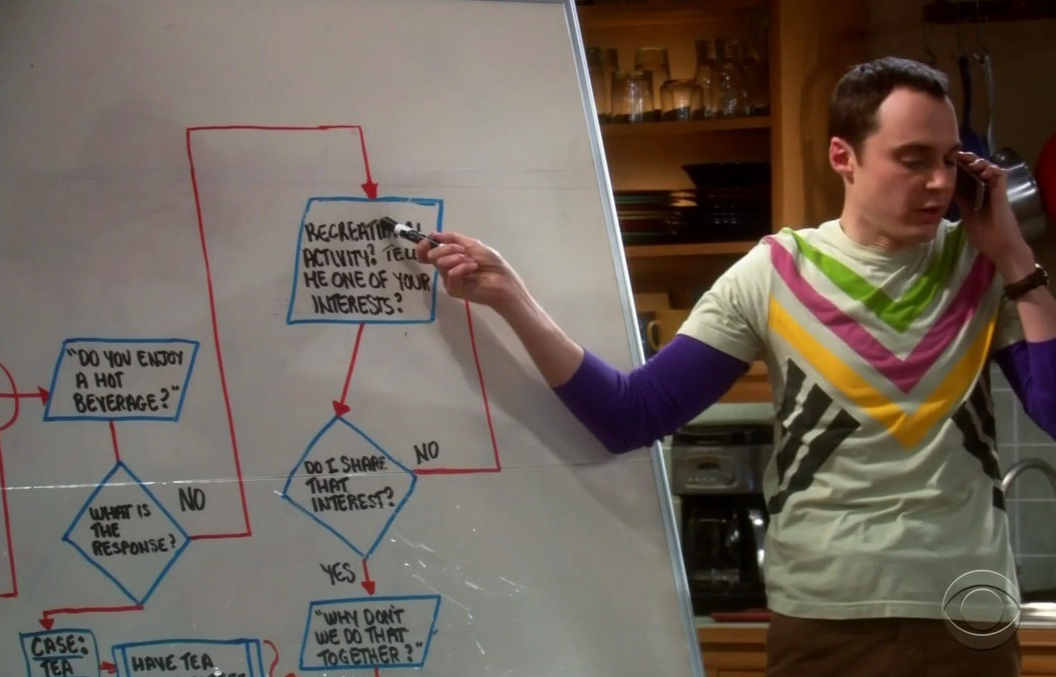
\includegraphics[width=7cm]{fig/Algorithm-sheldon.png}
            
                 \textit{ I believe I've isolateblblblblblblsblbslbslbsl
            sblbslblsblsblblsblbs
            lbslblbslsb d the algorithm for making friends.}
     
            
            \small{
            \hfill Sheldon Cooper, 
            
            \hfill in \textit{The Big Band Theory}, Season 2, Episode 13
            }
}

    \end{columns}

\end{frame}


%%%%%%%%%%%%%%%%%%%%%
\subsection{Introduction}
    \begin{frame}
    \frametitle{Pourquoi faire appel � des algorithmes ?}
    Pour automatiser des t�ches
    
    Exemples :
    \begin{itemize}
    \item M�tier � tisser\\
    \item M�thode de calcul � la main d'une division\\
    \item Recette de cuisine\\
    \item ...\\
    \end{itemize}
    \end{frame}
 
 %%%%%%%%%%%%%%%%%
 
    \begin{frame}
    \frametitle{Qu'est-ce qu'un algorithme ?}
    \begin{block}{D�finition}
    Un algorithme est un ensemble 
    ordonn� d'instructions simples
permettant de r�soudre un probl�me.
    \end{block}
    \end{frame}
    
 %%%%%%%%%%%%%%%%%%
 \subsection{Construction d'un algorithme}
%%%%%%%%%%%%%%%%%%%    
\section{La machine de Turing}
%%%%%%%%%%%%%%%%%%%%
 
  
\begin{frame}[fragile]
\frametitle{Un peu d'histoire...}
\begin{codeblock}{Test}
\begin{codeC}
for (int i = 0 ; i < n ; i ++) {
    //a comment
    printf("%d",i);
    }
\end{codeC}
\end{codeblock}

\begin{termblock}{test 2}
\lstset{escapeinside={��}}
\begin{lstlisting}
�\textbf{>>}�./a.out
�\color{darkgray}{\texttt{  Hello World}}�
\end{lstlisting}
\end{termblock}

 \begin{block}{Bloc standard}
blablabla
\end{block}
\end{frame}


\begin{frame}[fragile]
\frametitle{essai}
\begin{columns}
\column{6cm}
\begin{block}

\begin{figure}
\begin{tikzpicture} [
    auto,
    decision/.style = { diamond, draw=blue, thick, fill=blue!20,
                        text width=5em, text badly centered,
                        inner sep=1pt, rounded corners },
    block/.style    = { rectangle, draw=blue, thick, 
                        fill=blue!20, text width=10em, text centered,
                        rounded corners, minimum height=2em },
    line/.style     = { draw, thick, ->, shorten >=2pt },
  ]
   \matrix [column sep=-10mm, row sep=10mm] {
                    & \node [text centered] (x) {$\mathbf{X}$};            & \\
                    & \node (null1) {};                                    & \\
                    & \node [block] (doa) {\textsf{DoAE}($\mathbf{X}$)};   & \\
  	               \node(null3){}; & \node [decision] (uiddes)
                        {\textsf{UID}($\hat{\mathbf{X}}$)};
                                  & \node[text centered](tra){$\mathbf{i}$}; \\
                  & \node [block] (track) {\textsf{DoAT}($\mathbf{x}$)}; & \\
                    & \node [block] (pesos)
                        {\textsf{BF}(DoA$_{\mathrm{T}}$,DoAs)};            & \\
                    & \node [block] (filtrado)
                        {\textsf{SF}($\mathbf{w}$,$\mathbf{x}$)};          & \\
                    & \node [text centered] (xf) {$\hat{x}(t)$ };          & \\
  };
  % connect all nodes defined above
 \begin{scope} [every path/.style=line]
    \path (x)        --    (doa);
    \path (doa)      --    node [near start] {DoAs} (uiddes);
    \path (tra)      --    (uiddes);
    \path (uiddes)   --++  (-3,0) node [near start] {no} |- (null1);
    \path (uiddes)   --    node [near start] {DoA} (track);
    \path (track)    --    node [near start] {DoA$_{\mathrm{T}}$} (pesos);
    \path (pesos)    --    node [near start] {\textbf{w}} (filtrado);
    \path (filtrado) --    (xf);
  
  \end{scope}
\end{tikzpicture}
\end{figure}
\end{block}
\column{3cm}
\begin{block}{bulbul}
\end{block}
\end{columns}
\end{frame}

\end{document}
